
%(BEGIN_QUESTION)
% Copyright 2007, Tony R. Kuphaldt, released under the Creative Commons Attribution License (v 1.0)
% This means you may do almost anything with this work of mine, so long as you give me proper credit

Qualitatively graph the response of a direct-acting I-only controller:

$$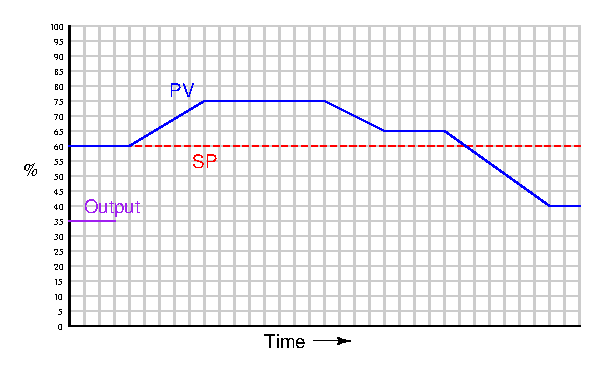
\includegraphics[width=15.5cm]{i01850x01.eps}$$

Qualitatively graph the response of a direct-acting P+I controller:

$$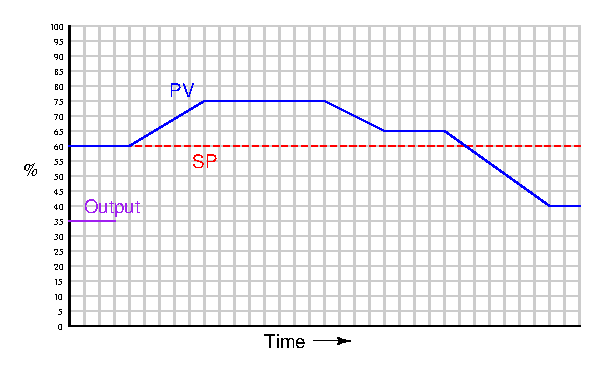
\includegraphics[width=15.5cm]{i01850x01.eps}$$

Qualitatively graph the response of a direct-acting P+I+D controller:

$$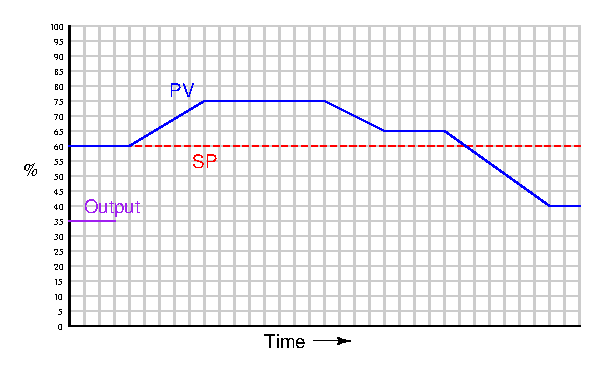
\includegraphics[width=15.5cm]{i01850x01.eps}$$

\underbar{file i01850}
%(END_QUESTION)





%(BEGIN_ANSWER)

I recommend deducting 0.5 point for each incorrectly-shaped segment of the output line in each graph.  This way, students can still get partial credit even if one or more of the initial segments is drawn incorrectly:

$$\includegraphics[width=15.5cm]{i01850x02.eps}$$

$$\includegraphics[width=15.5cm]{i01850x03.eps}$$

$$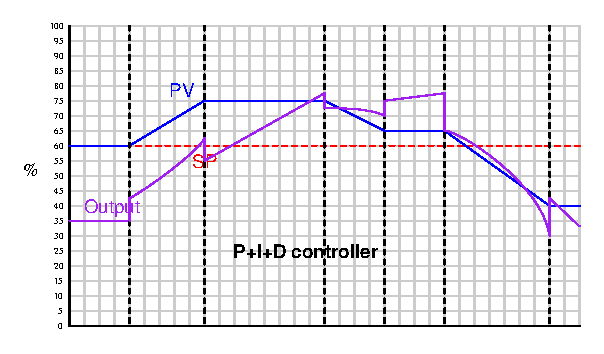
\includegraphics[width=15.5cm]{i01850x04.eps}$$

%(END_ANSWER)





%(BEGIN_NOTES)

{\bf This question is intended for exams only and not worksheets!}.

%(END_NOTES)


